\subsection{Loop ordering}\label{sec:loopordering}
A blocked implementation of matrix multiplication contains a series of nested
loops; one of the optimizations we attempted was the reordering of these loops.
A blocked implementation has two different places where the loop ordering can
be changed: the order in which the blocks are processed (i.e. outside loop
ordering), and the ordering inside of each block multiplication (i.e. inside
loop ordering).

\subsubsection{Inside Loop Ordering}
When multiplying blocks, we see that there are three index variables: $i$, $j$,
and $k$ associated with the three loops. Changing the ordering of these loops
affects the stride and regularity at which we access memory, which can have a
significant effect upon performance. For example, striding down the column of a
row-major matrix is less efficient that striding across the row because the
longer stride has less spatial locality and fits poorly in cache.

We note that there are $3! = 6$ possible orderings of these loops. In order to
determine which was fastest, we tested and compared all 6 on the totient node.
Note that we kept the outside loop ordering constant for all of these, as we
assumed that the inside and outside loop orderings were orthogonal, or at least
close enough that the difference was not significant. The results can be found
in \figref{insideloop}. We see that the loop ordering of $j,k,i$ was
clearly fastest, and significantly faster than the slowest loop orderings.

\begin{figure}[hh]
  \centering
  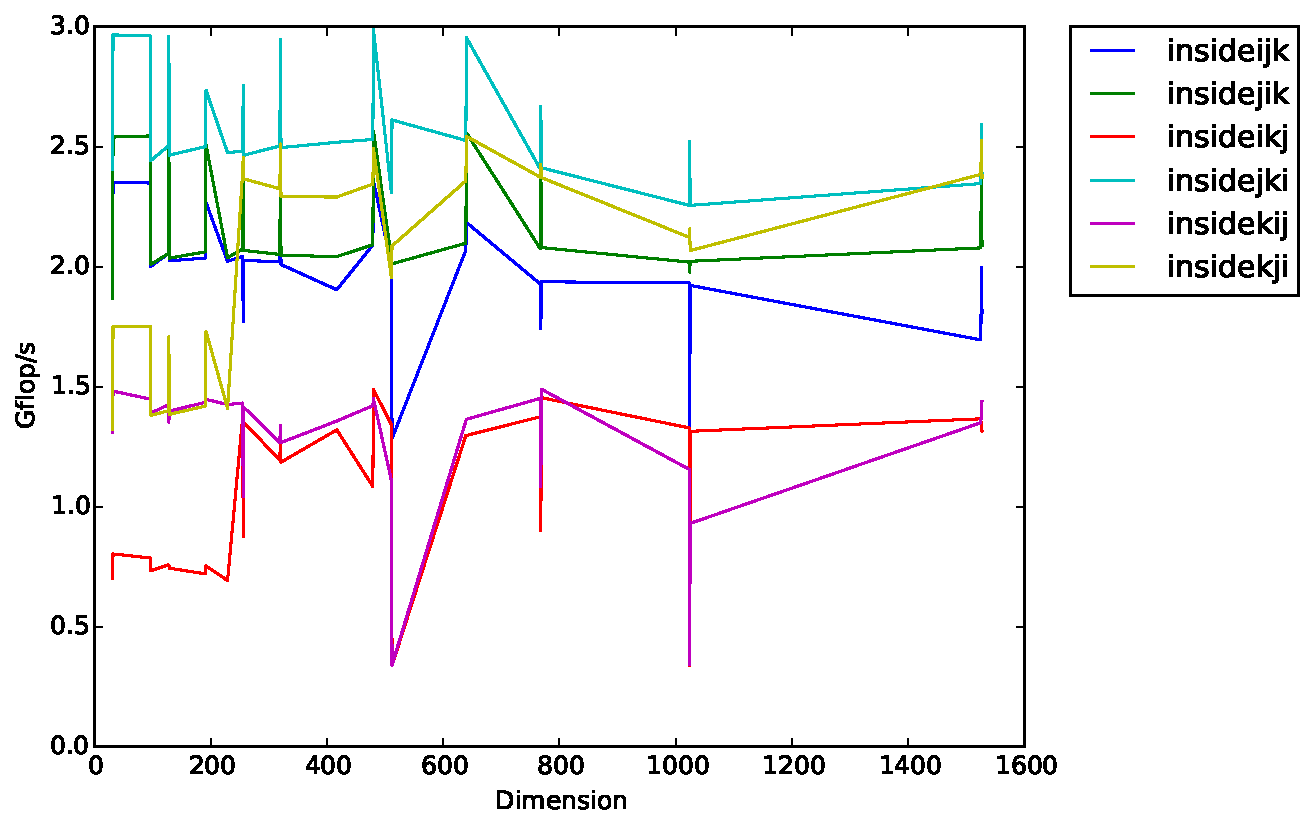
\includegraphics[width=\textwidth]{img/timing_insideloops.pdf}
  \caption{Timing results for the different inside loop orderings}
  \label{fig:insideloop}
\end{figure}

\subsubsection{Outside Loop Ordering}
Similarly, we can also change the order in which we multiply blocks. Again, we
compared the six different possible orderings, while keeping the inside loop
ordering fixed as $j,k,i$, which was found to be the fastest in the previous
subsection. The timing results are found in \figref{outsideloop}.

We see that some loop orderings are definitely faster than others, but unlike
with the inside loop orderings, there is no clear best ordering as both $k,j,i$
and $i,k,j$ are fastest on different size matrices. We chose to go with the
outside loop ordering $i,k,j$

\begin{figure}[hh]
  \centering
  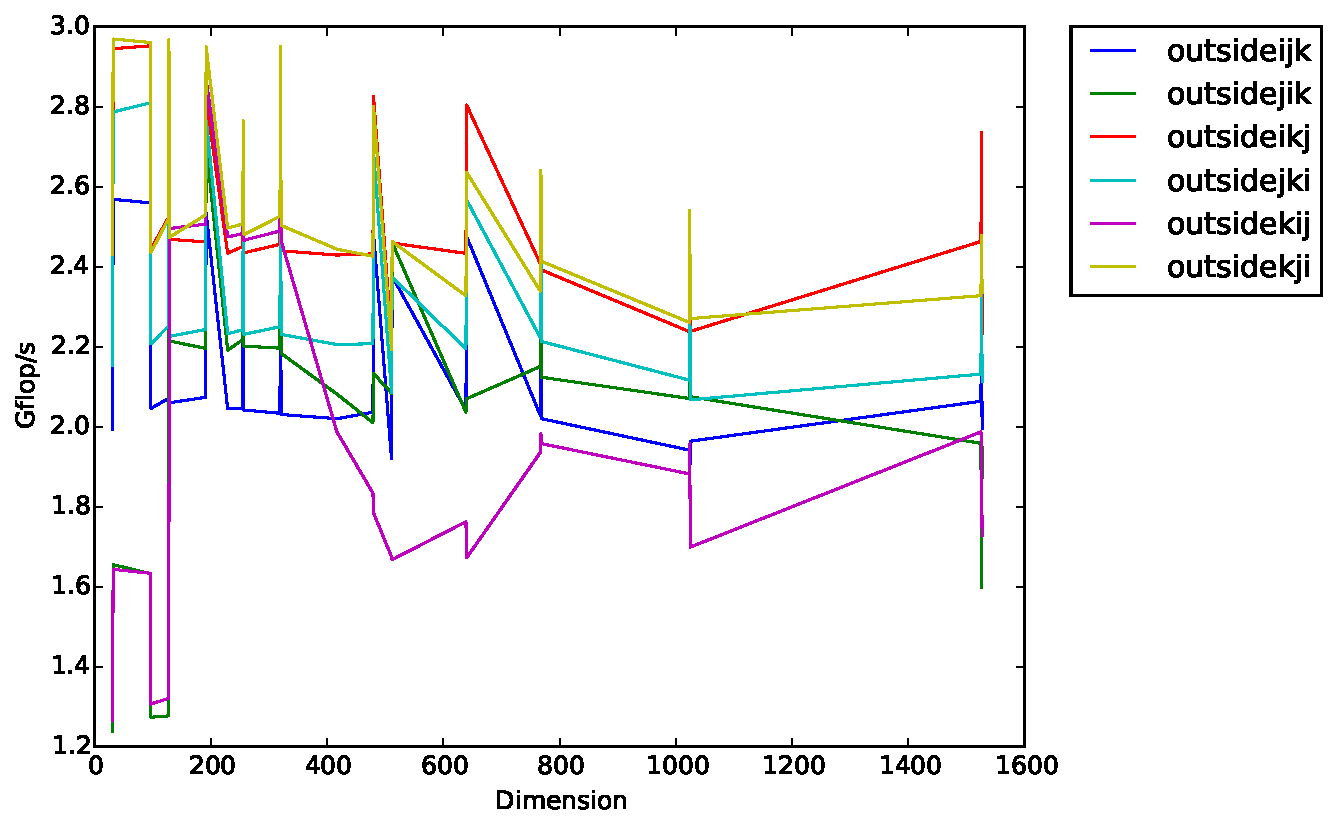
\includegraphics[width=\textwidth]{img/timing_outsideloops.pdf}
  \caption{Timing results for the different outside loop orderings}
  \label{fig:outsideloop}
\end{figure}
